
% Tamoanchan Revisited chapter ========================================
\chapter*{Tamoanchan Revisited}
\addcontentsline{toc}{chapter}{Tamoanchan Revisited}

\begin{flushright}
\parbox{0.6\textwidth}{
\emph{I dream, therefore I exist. \\
\hspace*{\fill}{\textperiodcentered \textperiodcentered \textperiodcentered \hspace*{0.2em} August Strindberg} } }
\end{flushright}

\noindent
Tamoanchan Revisited is chess variant which is played on 22 x 22 board,
with white and bright cyan fields and light grey and grey pieces.
Star colors are yellow and bright red. In algebraic notation, columns
are enumerated from 'a' to 'v', and rows are enumerated from '1' to '22'.
A new piece is introduced, Serpent.

\clearpage % ..........................................................
% Serpent *************************************************************

\section*{Serpent}
\addcontentsline{toc}{section}{Serpent}

\noindent
\begin{wrapfigure}[10]{l}{0.4\textwidth}
\centering
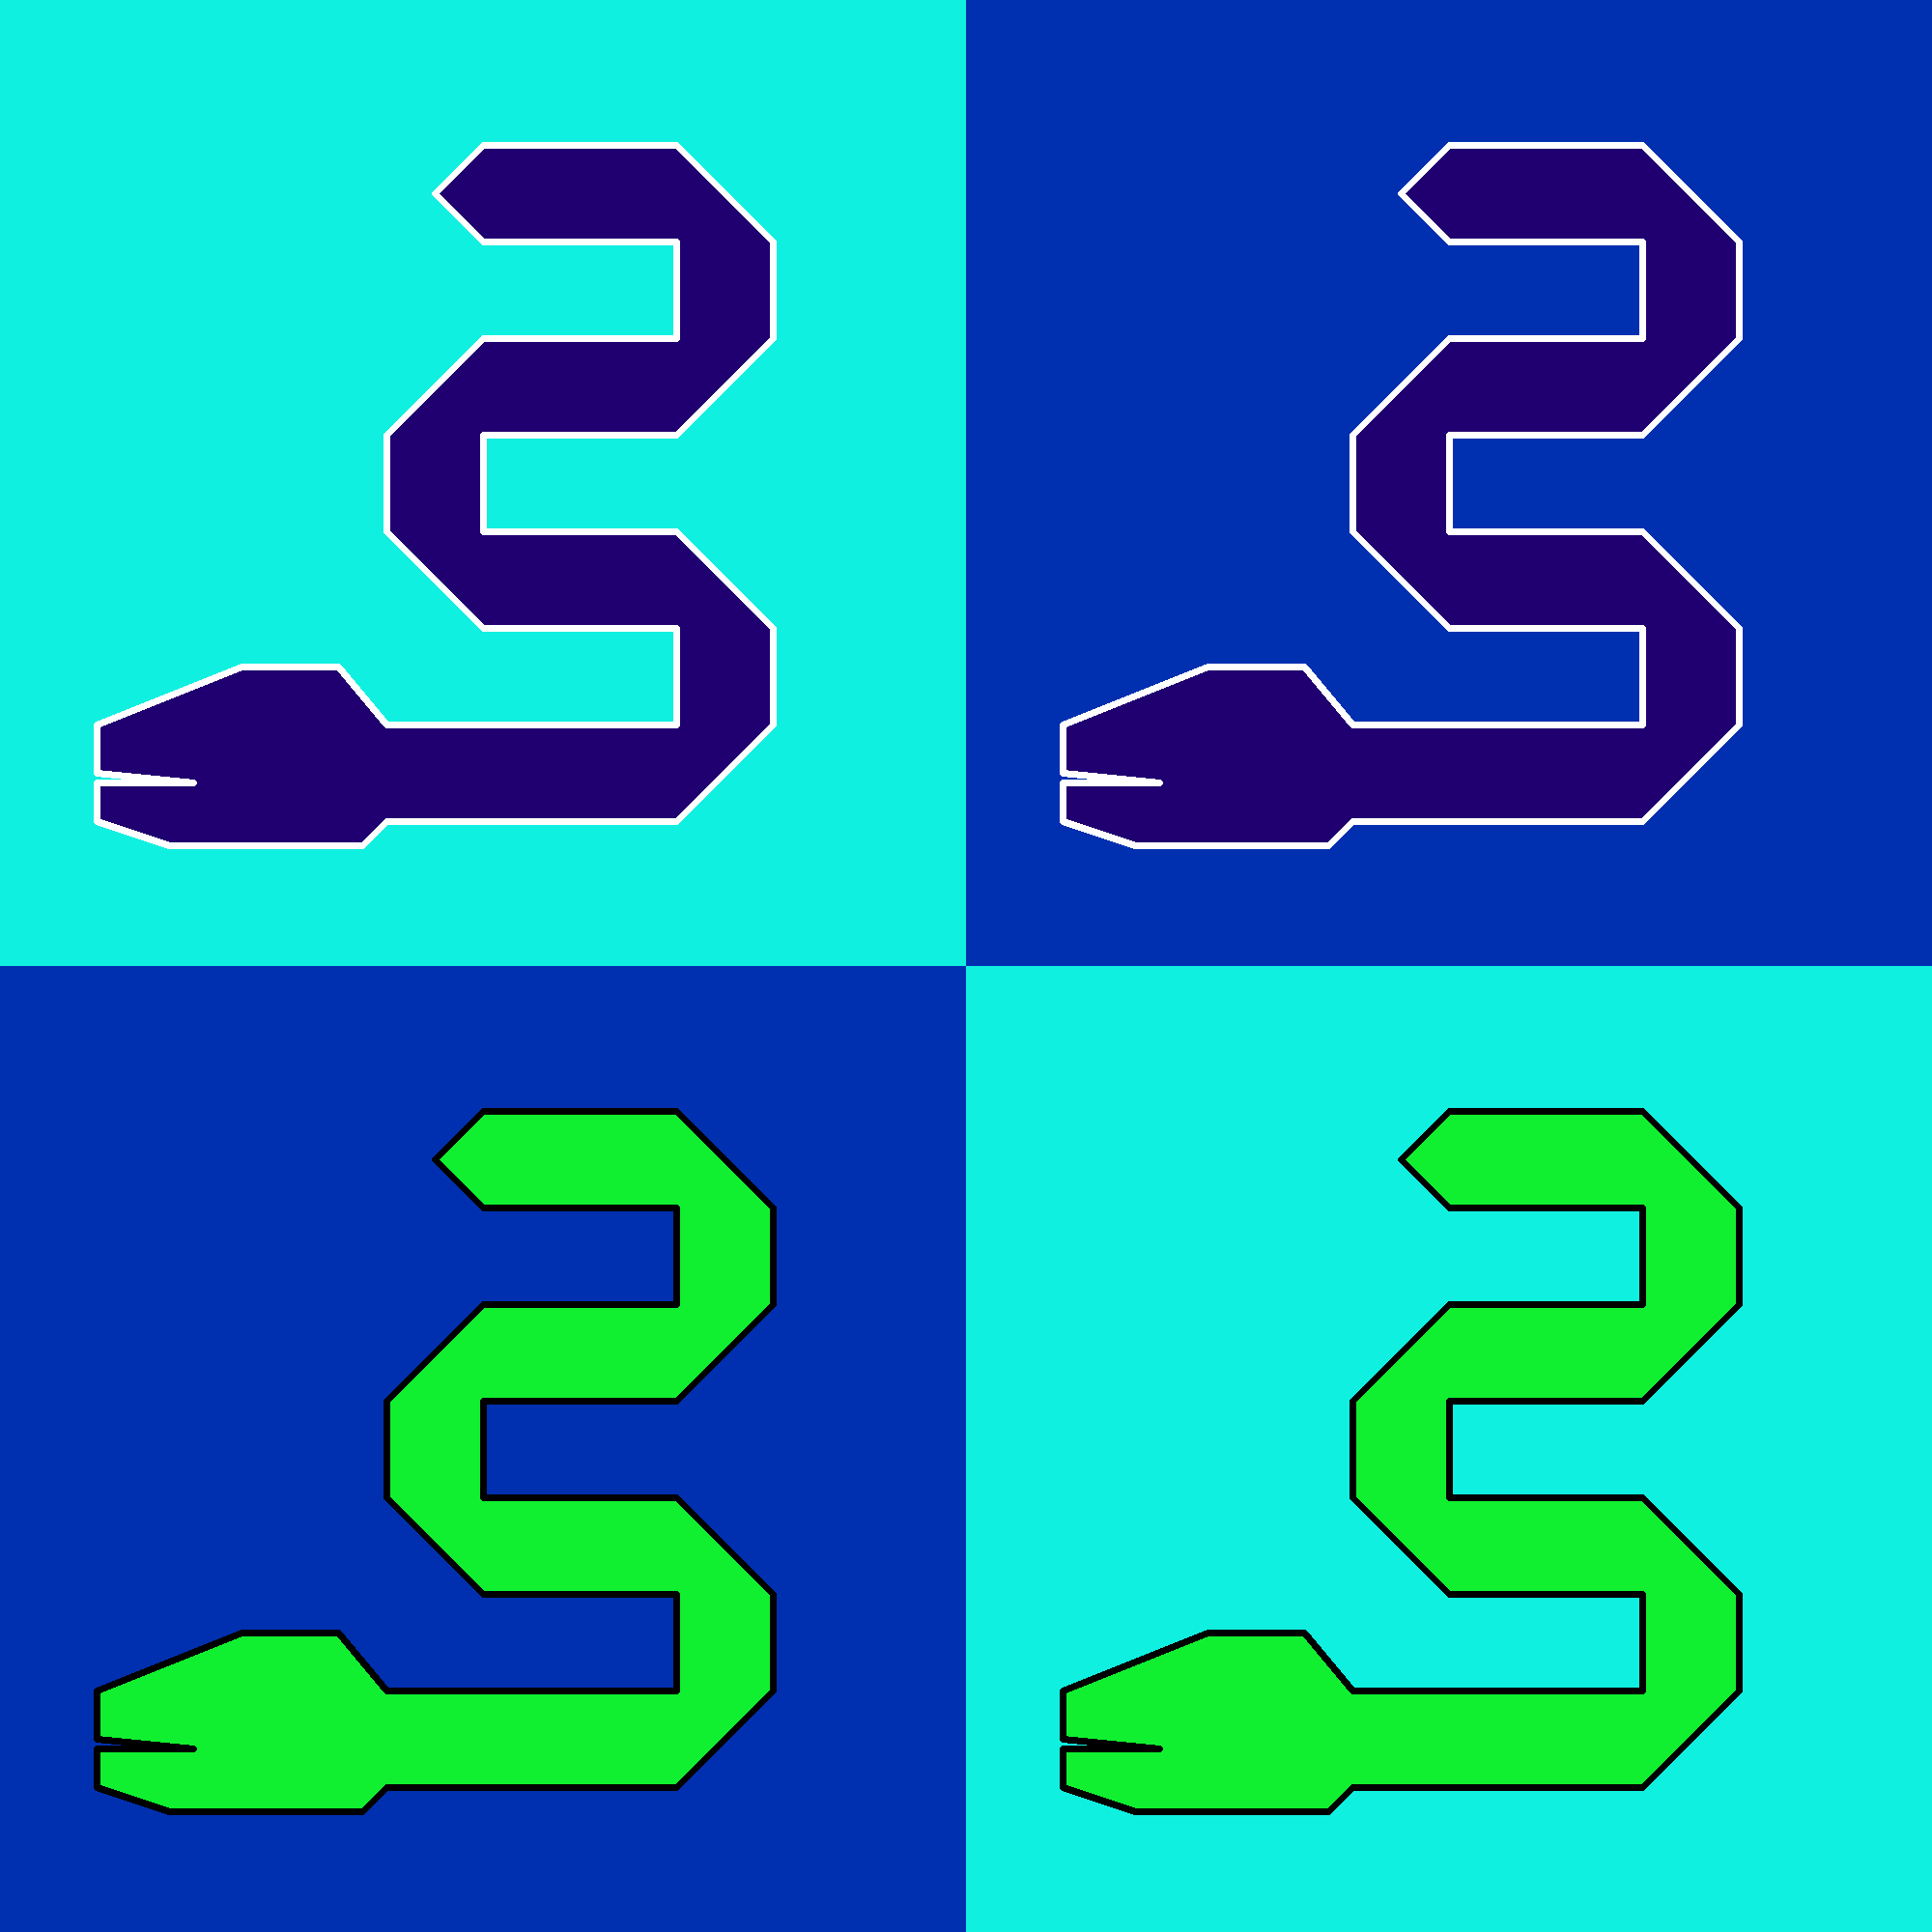
\includegraphics[width=0.4\textwidth, keepaspectratio=true]{pieces/13_serpent.png}
\caption{Serpent}
\label{fig:13_serpent}
\end{wrapfigure}
Serpent moves diagonaly one field at the time, after which it alternates
diagonal.

Serpent can also move one field vertically or horizontaly if it's unoccupied.
This move is complete move of a player, and cannot contain anything else.

In algebraic notation symbol for Serpent is ’S’.

% \vspace*{0.05\textheight}
\noindent
\begin{wrapfigure}{l}{0.4\textwidth}
\centering
\includegraphics[width=0.4\textwidth, keepaspectratio=true]{pieces/star/16_tamoanchan_revisited.png}
\caption{Star}
\label{fig:star/16_tamoanchan_revisited}
\end{wrapfigure}
Star colors in this variant are presented to the left.

% ************************************************************* Serpent
\clearpage % ..........................................................

\section*{Promotion}
\addcontentsline{toc}{section}{Promotion}

Promotion is non enforced, delayed variety, i.e. it's the same as in
\hyperref[sec:Age of Aquarius/Promotion]{previous chess variant}, Age of Aquarius.

Promotion in this variant is polygamous, more than one Queen in the same color
can be present on chessboard at any given time.

\clearpage % ..........................................................

\section*{En passant}
\addcontentsline{toc}{section}{En passant}

\noindent
\begin{wrapfigure}{l}{0.4\textwidth}
\centering
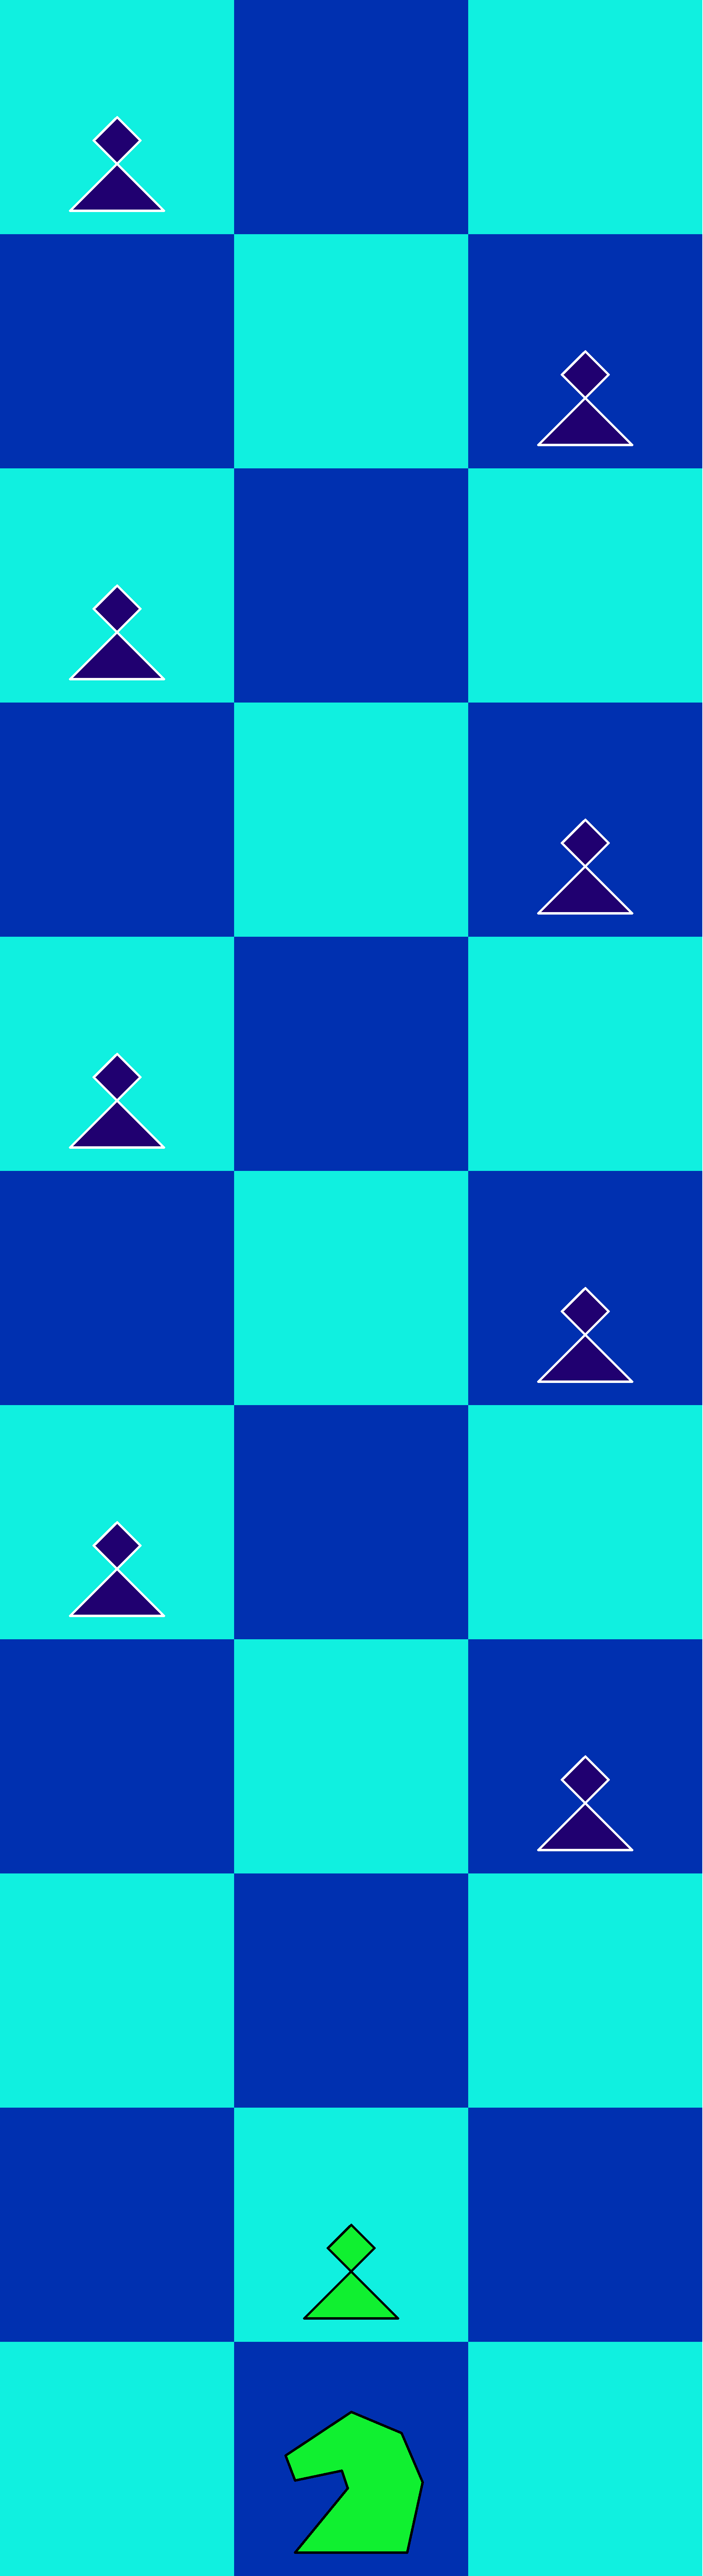
\includegraphics[width=0.15\textwidth, keepaspectratio=true]{en_passants/16_tamoanchan_revisited_en_passant.png}
\caption{En passant}
\label{fig:16_tamoanchan_revisited_en_passant}
\end{wrapfigure}
Rush and en passant are identical to those in Classic Chess, only difference
is that Pawn can now move longer on initial turn, up to 9 fields in this
variant.

\clearpage % ..........................................................

\section*{Castling}
\addcontentsline{toc}{section}{Castling}

Castling is the same as in Classical Chess, only difference is that King can move between 2 and 8 fields across.
All other constraints from Classical Chess still applies.

\noindent
\begin{figure}[!h]
% \begin{figure}[!t]
\includegraphics[width=1.0\textwidth, keepaspectratio=true]{castlings/16_tr/tamoanchan_revisited_castling.png}
\caption{Castling}
\label{fig:tamoanchan_revisited_castling}
% \centering
\end{figure}

In example above, all valid King's castling moves are numbered.

\noindent
\begin{figure}[!h]
% \begin{figure}[!t]
\includegraphics[width=1.0\textwidth, keepaspectratio=true]{castlings/16_tr/tamoanchan_revisited_castling_left_03.png}
\caption{Castling short left}
\label{fig:tamoanchan_revisited_castling_left_03}
% \centering
\end{figure}

In this example King was castling short to the left. Initial King's position is marked with "K".
After castling is finished, left Rook ends up at field immediately right to the King.

\clearpage % ..........................................................

\section*{Initial setup}
\addcontentsline{toc}{section}{Initial setup}

Initial setup can be seen in image below:

\noindent
% \begin{figure}[t]
\begin{figure}[h]
\includegraphics[width=1.0\textwidth, keepaspectratio=true]{boards/16_tamoanchan_revisited.png}
\caption{Tamoanchan Revisited board}
\label{fig:16_tamoanchan_revisited}
% \centering
\end{figure}

\clearpage % ..........................................................
% ======================================== Tamoanchan Revisited chapter
